
%%%%%%%%%%%%%%%%%%%%%%%%%%%%%%%%%%%%%%%%%%%%%%%%%%%%%%%%%%%%%%%%%%%%%%%%%%%%%%%%%%%%%%%%%%
\begin{frame}{Context : KoroiBot project}
\vspace*{-1.0cm}
\begin{center}
  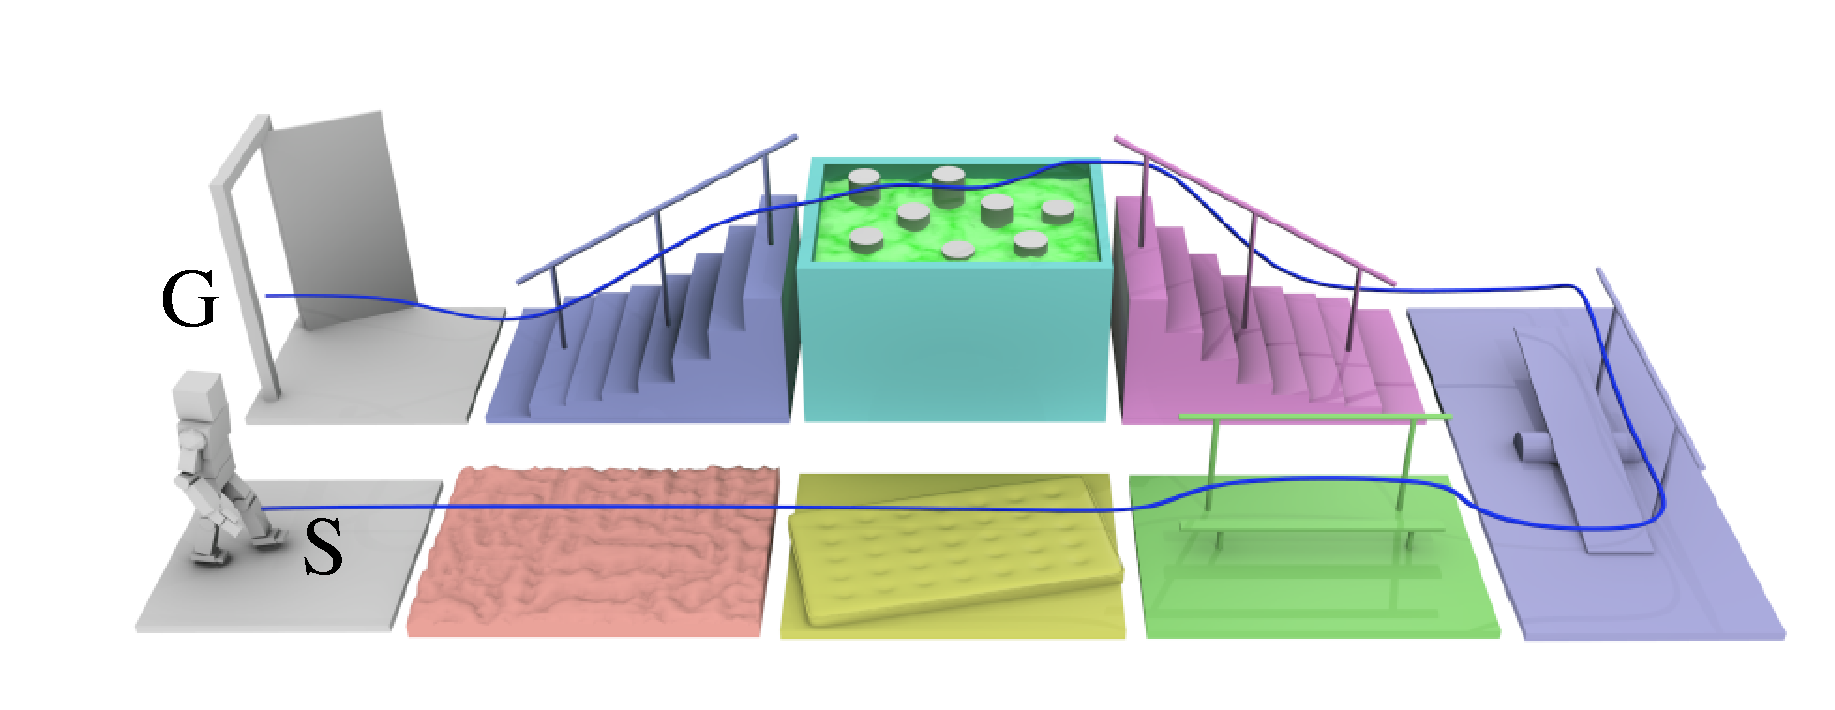
\includegraphics[width=\linewidth]{koroibot/KoroibotChallengeEnhanced.pdf}
  \begin{tikzpicture}[remember picture, overlay]
%    \draw[help lines] (0,0) grid (-1,1);
%    \node at (0,0) {(0,0)};
    \draw[line width=1.5pt, color=red](-10,1) ellipse (0.8cm and .6cm);
    \draw[line width=1.5pt, color=red](-8,1) ellipse (1.1cm and .6cm);
    \draw[line width=1.5pt, color=red](-3.3,1) ellipse (1.1cm and .6cm);
    \draw[line width=1.5pt, color=red](-3.5,3) ellipse (1.0cm and .8cm);
    \draw[line width=1.5pt, color=red](-7.7,3) ellipse (1.0cm and .8cm);
    \draw[line width=1.5pt, color=red](-5.7,3) circle (1.0cm);
  \end{tikzpicture}
\end{center}
%\begin{itemize}
%  \item 
%\end{itemize}
Goal : enhance the ability of humanoid robots to walk in a dynamic and versatile way, and to bring them closer to human capabilities.
\end{frame}
%%%%%%%%%%%%%%%%%%%%%%%%%%%%%%%%%%%%%%%%%%%%%%%%%%%%%%%%%%%%%%%%%%%%%%%%%%%%%%%%%%%%%%%%%%%

\begin{frame}{Project Partners}
\vspace*{-0.7cm}
\begin{columns}
\column{0.6\linewidth}
\begin{center}
  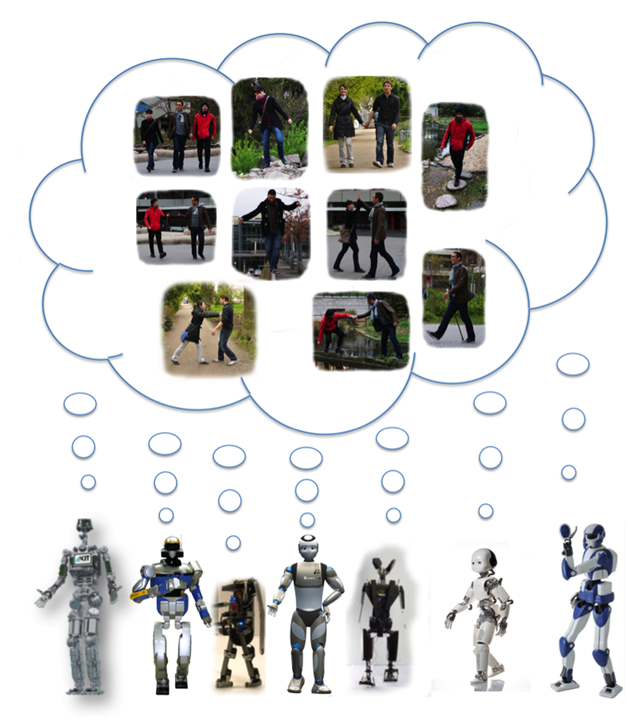
\includegraphics[height=0.75\textheight]{koroibot/situations_v2.png}
\end{center}
\vspace*{-0.5cm}
  \small{ \hspace*{0.3cm} ARMAR-IV \hspace*{0.4cm}  Leo \hspace*{0.4cm} TUlip \hspace*{0.6cm} HRP-4 }\\
  \small{ \hspace*{1.7cm} \textcolor{blue!50!black}{\textbf{HRP-2}} \hspace*{0.1cm} \textcolor{blue!50!black}{\textbf{Romeo}} \hspace*{0.3cm} iCube}
\column{0.4\linewidth}
\begin{center}
  
\includegraphics[height=0.1\textheight]{koroibot/logos/cnrs.png}\\
  
\includegraphics[height=0.1\textheight]{koroibot/logos/iit.png}\\
  
\includegraphics[height=0.1\textheight]{koroibot/logos/tud.png}\\
  
\includegraphics[height=0.1\textheight]{koroibot/logos/hd.png}\\
  
\includegraphics[height=0.1\textheight]{koroibot/logos/kit.png}\\
  
\includegraphics[height=0.1\textheight]{koroibot/logos/ut.png}\\
  
\includegraphics[height=0.1\textheight]{koroibot/logos/wi.png}
\end{center}

\end{columns}
%\begin{itemize}
%  \item 
%\end{itemize}
\end{frame}
%%%%%%%%%%%%%%%%%%%%%%%%%%%%%%%%%%%%%%%%%%%%%%%%%%%%%%%%%%%%%%%%%%%%%%%%%%%%%%%%%%%%%%%%%%
\begin{frame}{Key Performance Indicators}
  \begin{center}
    \movie[autostart,loop]{
    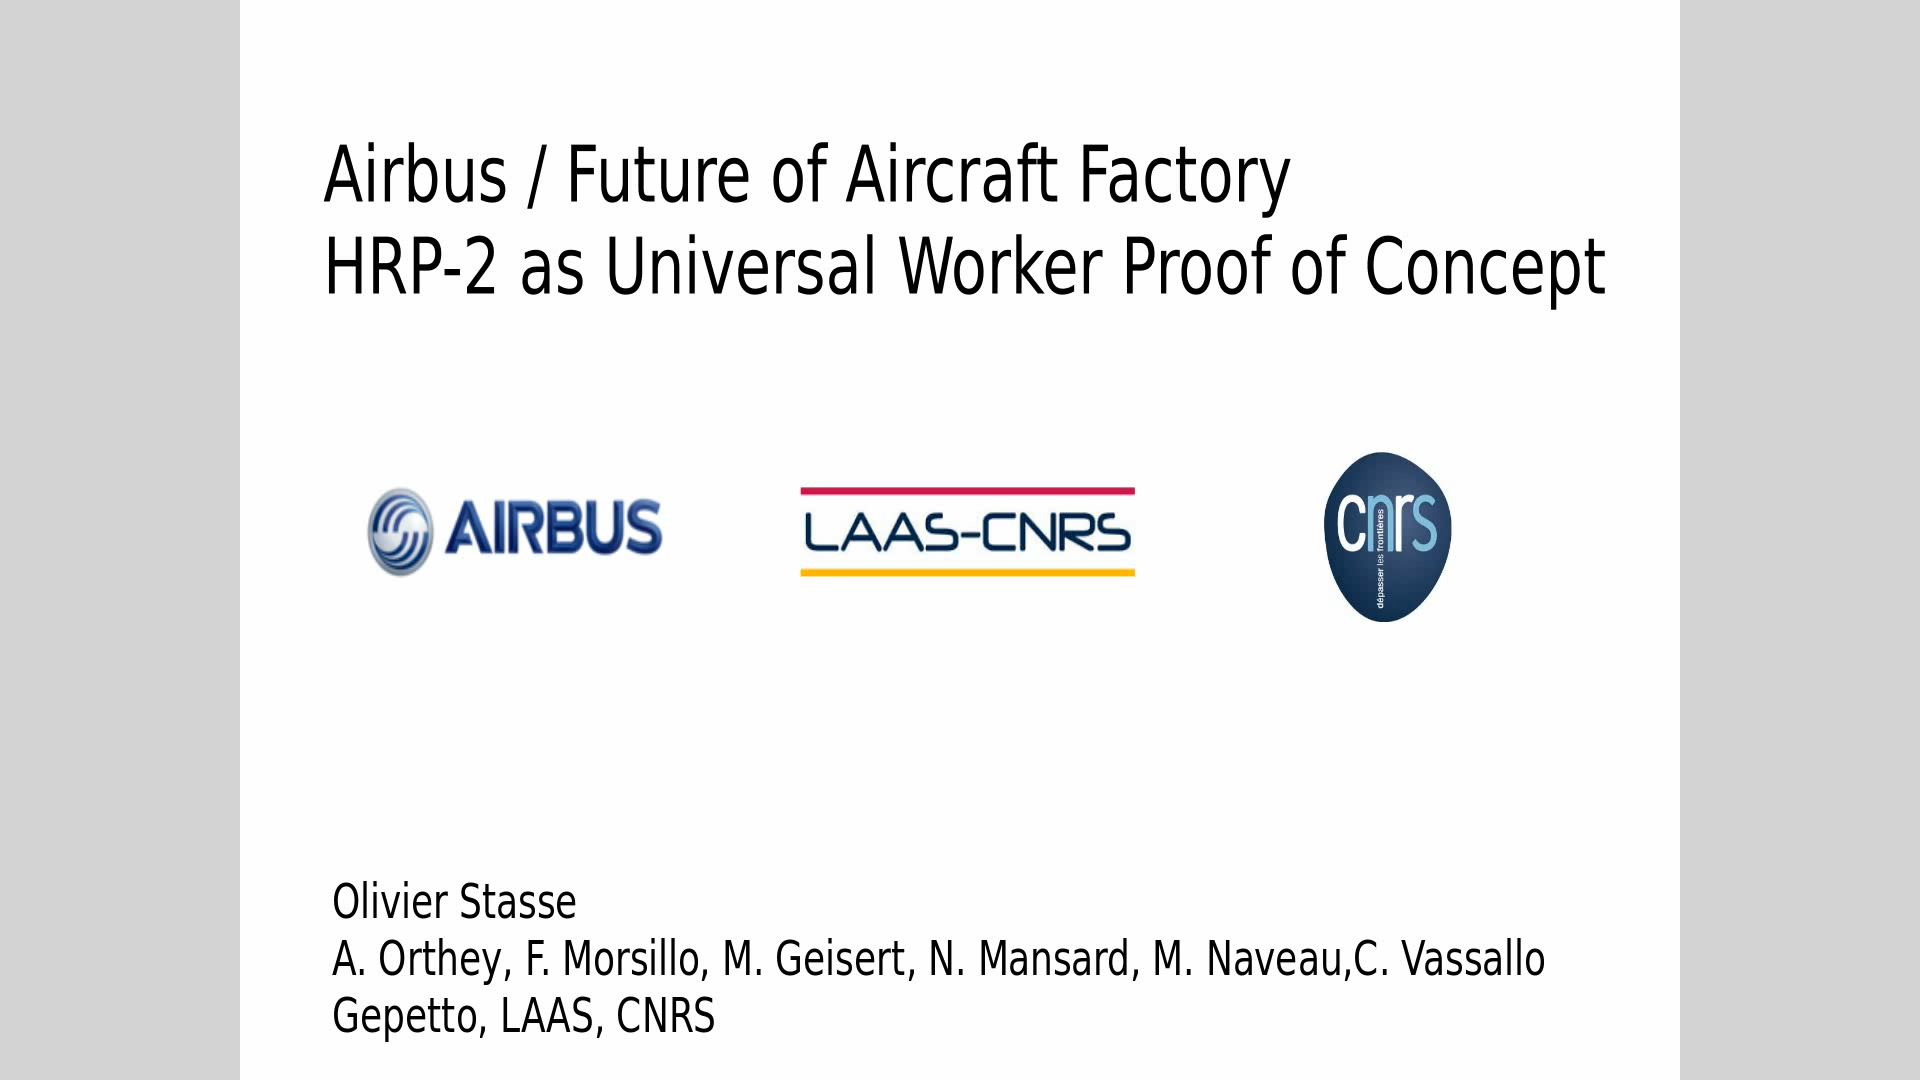
\includegraphics[width=0.3\linewidth, keepaspectratio]
      {poc_airbus/PocAirbus2013_12_Short.png}    
    }  
    {./videos/Koroibot-HRP2-GoingUp15cmLateralView.avi}
    \movie[autostart,loop]{
    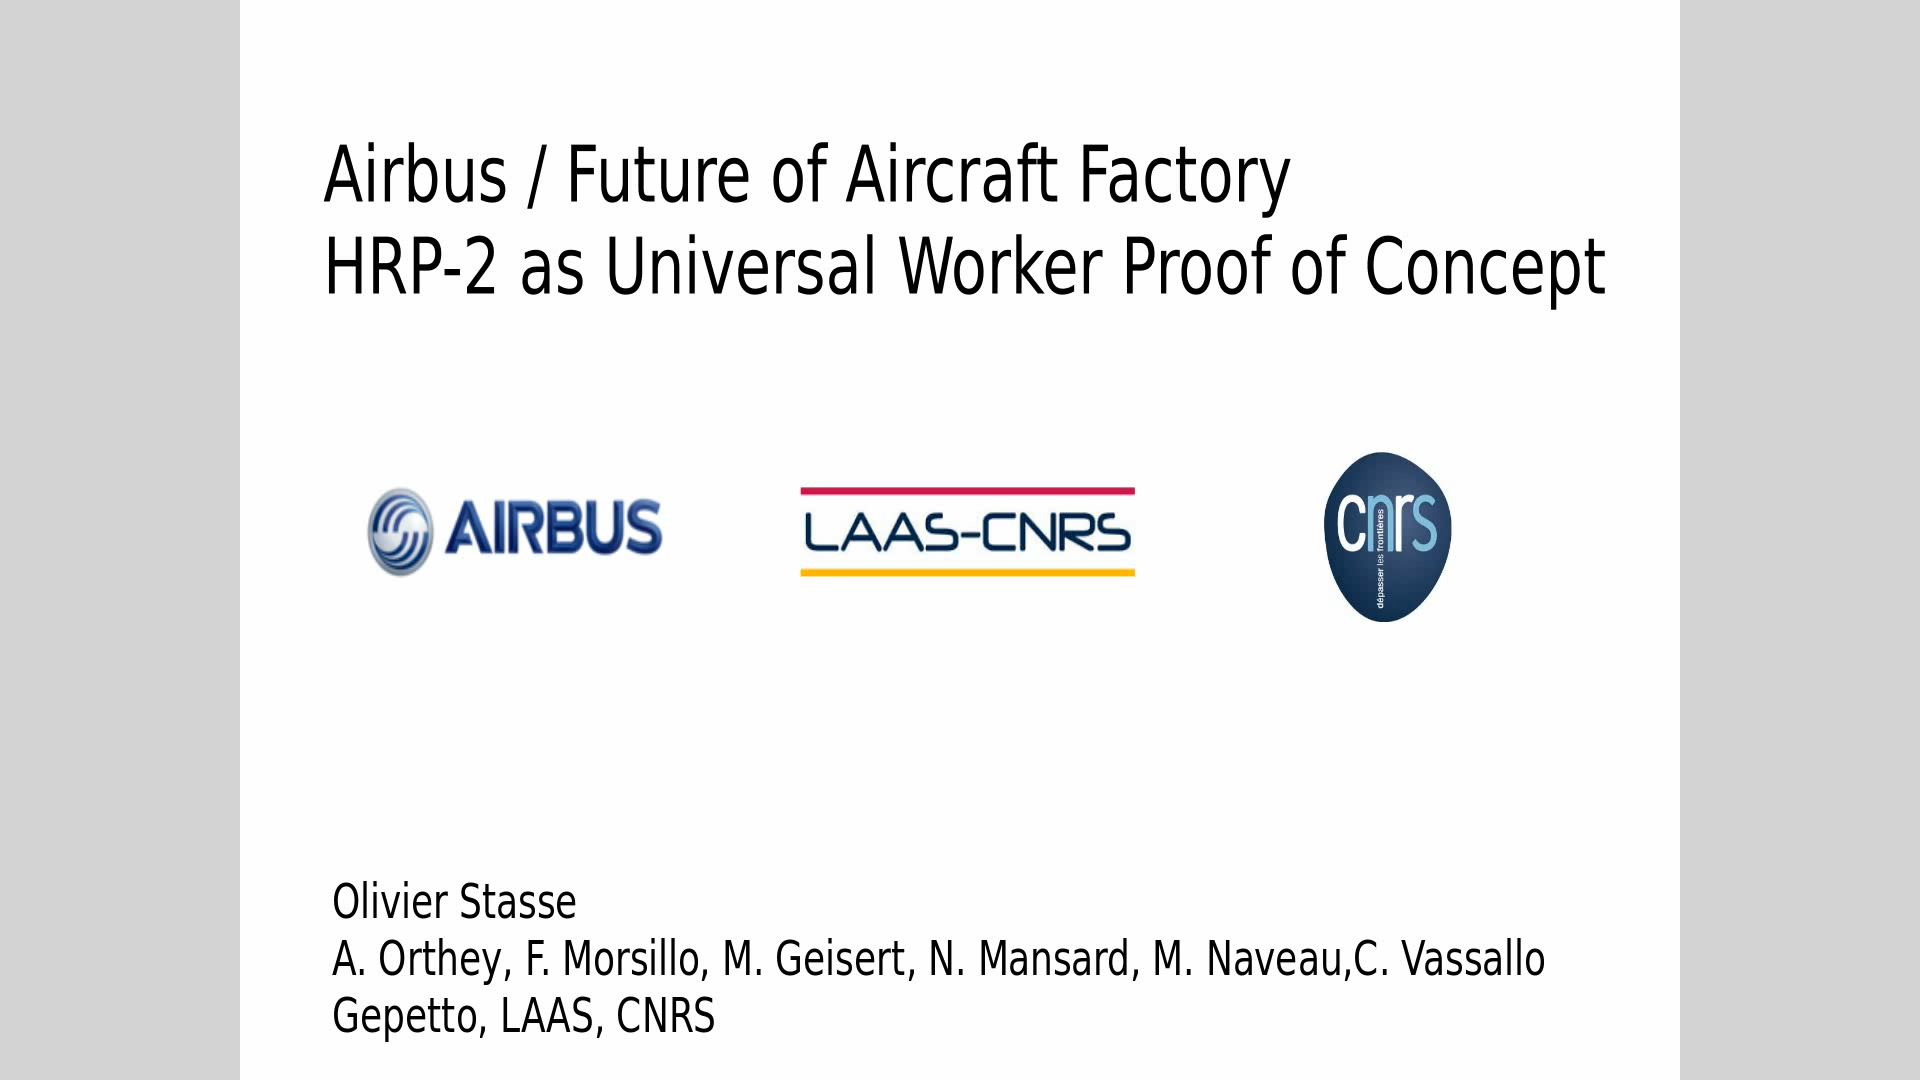
\includegraphics[width=0.3\linewidth, keepaspectratio]
      {poc_airbus/PocAirbus2013_12_Short.png}    
    }
    {./videos/Koroibot-HRP2-GoingUp10cmLateralViewv2.avi}
    \movie[autostart,loop]{
    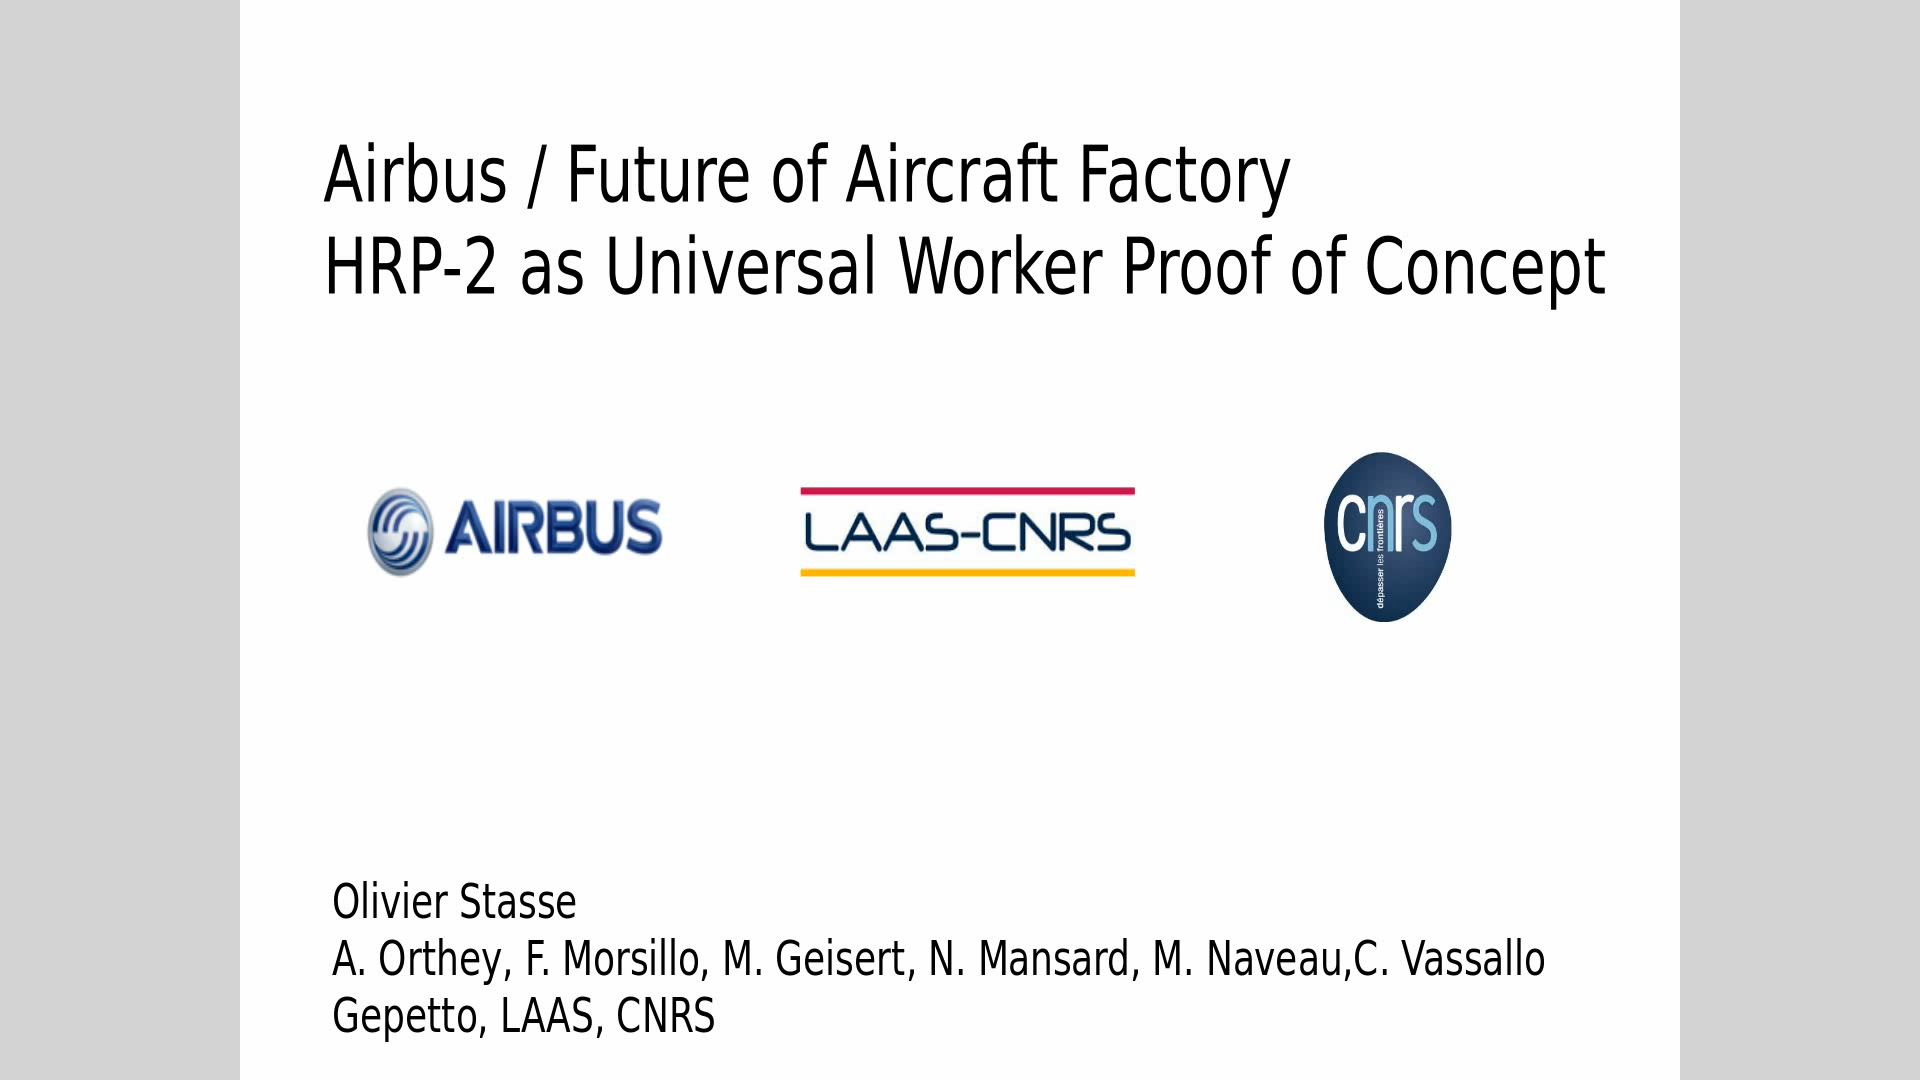
\includegraphics[width=0.3\linewidth, keepaspectratio]
      {poc_airbus/PocAirbus2013_12_Short.png}    
    }  
    {./videos/Koroibot-HRP2-SteppingStonesLateralView.avi}
    \movie[autostart,loop]{ 
    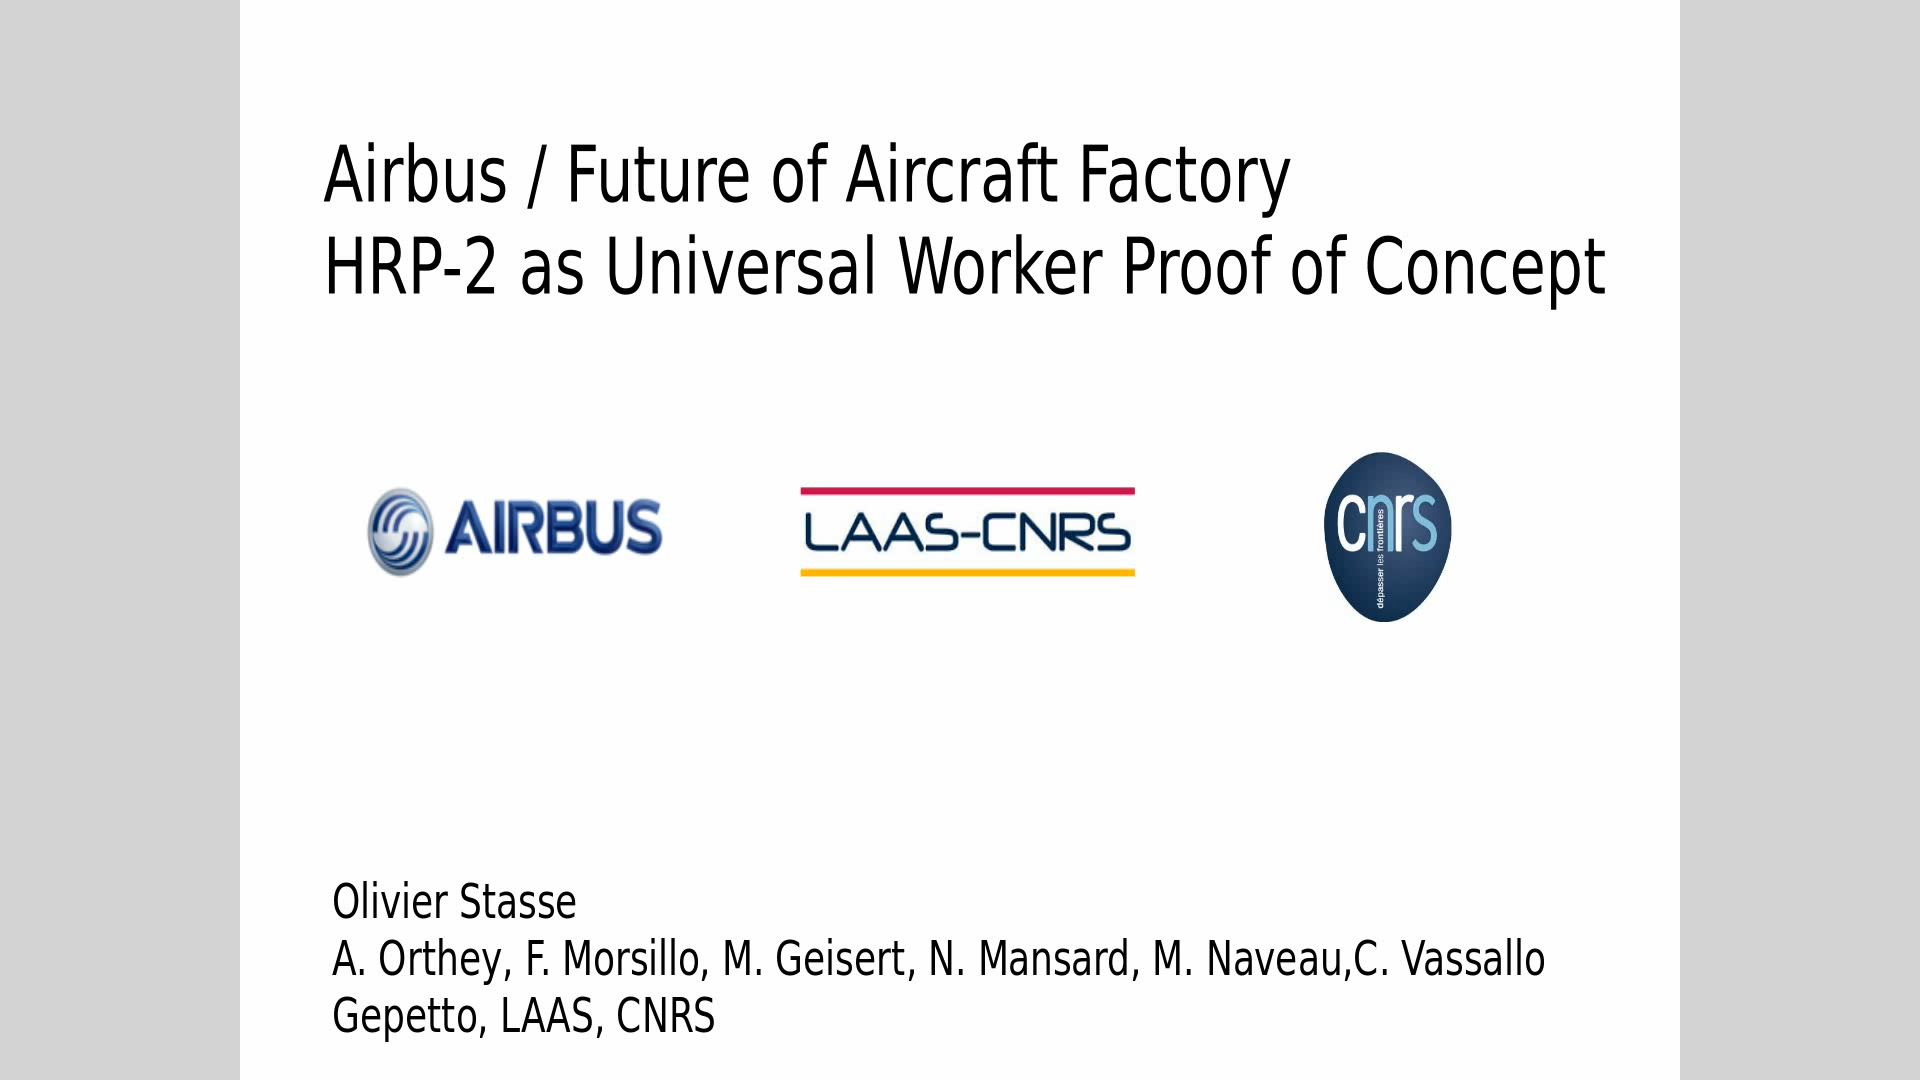
\includegraphics[width=0.3\linewidth, keepaspectratio]
      {poc_airbus/PocAirbus2013_12_Short.png}    
    }  
    {./videos/Koroibot-HRP2-WalkingOnBeam_v3.mp4}
    \movie[autostart,loop]{
    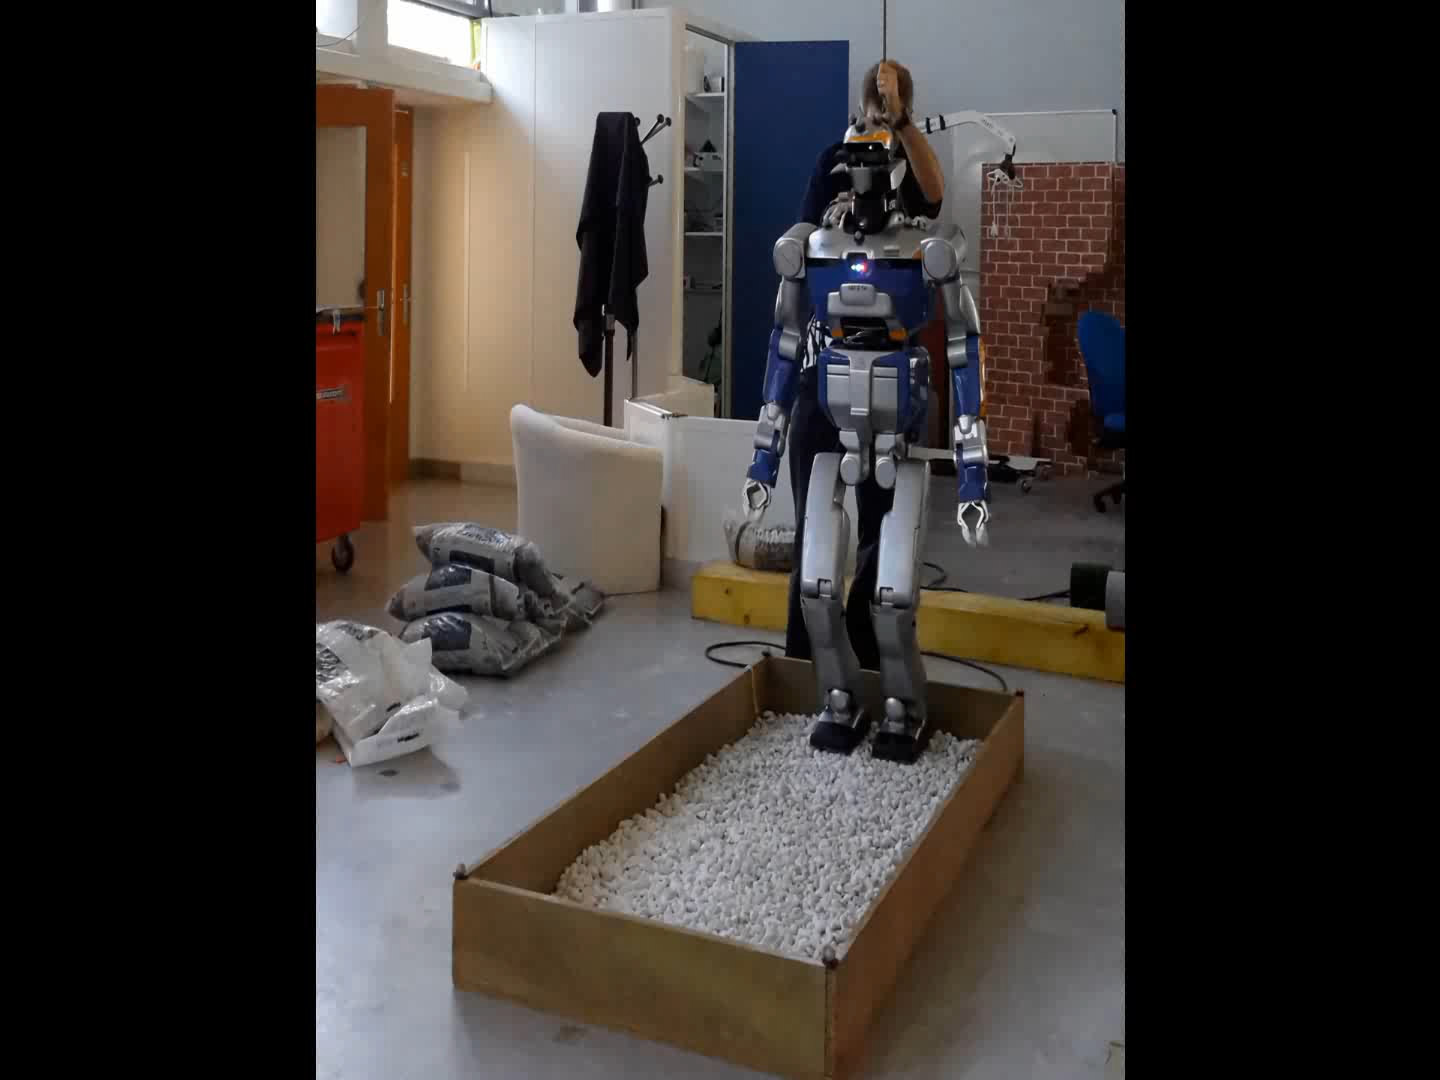
\includegraphics[width=0.3\linewidth, height=2.0cm]
      {koroibot/gravlekpi.png}    
    }  
    {./videos/Koroibot-gravle-rotate.mp4}
    \movie[autostart,loop]{
    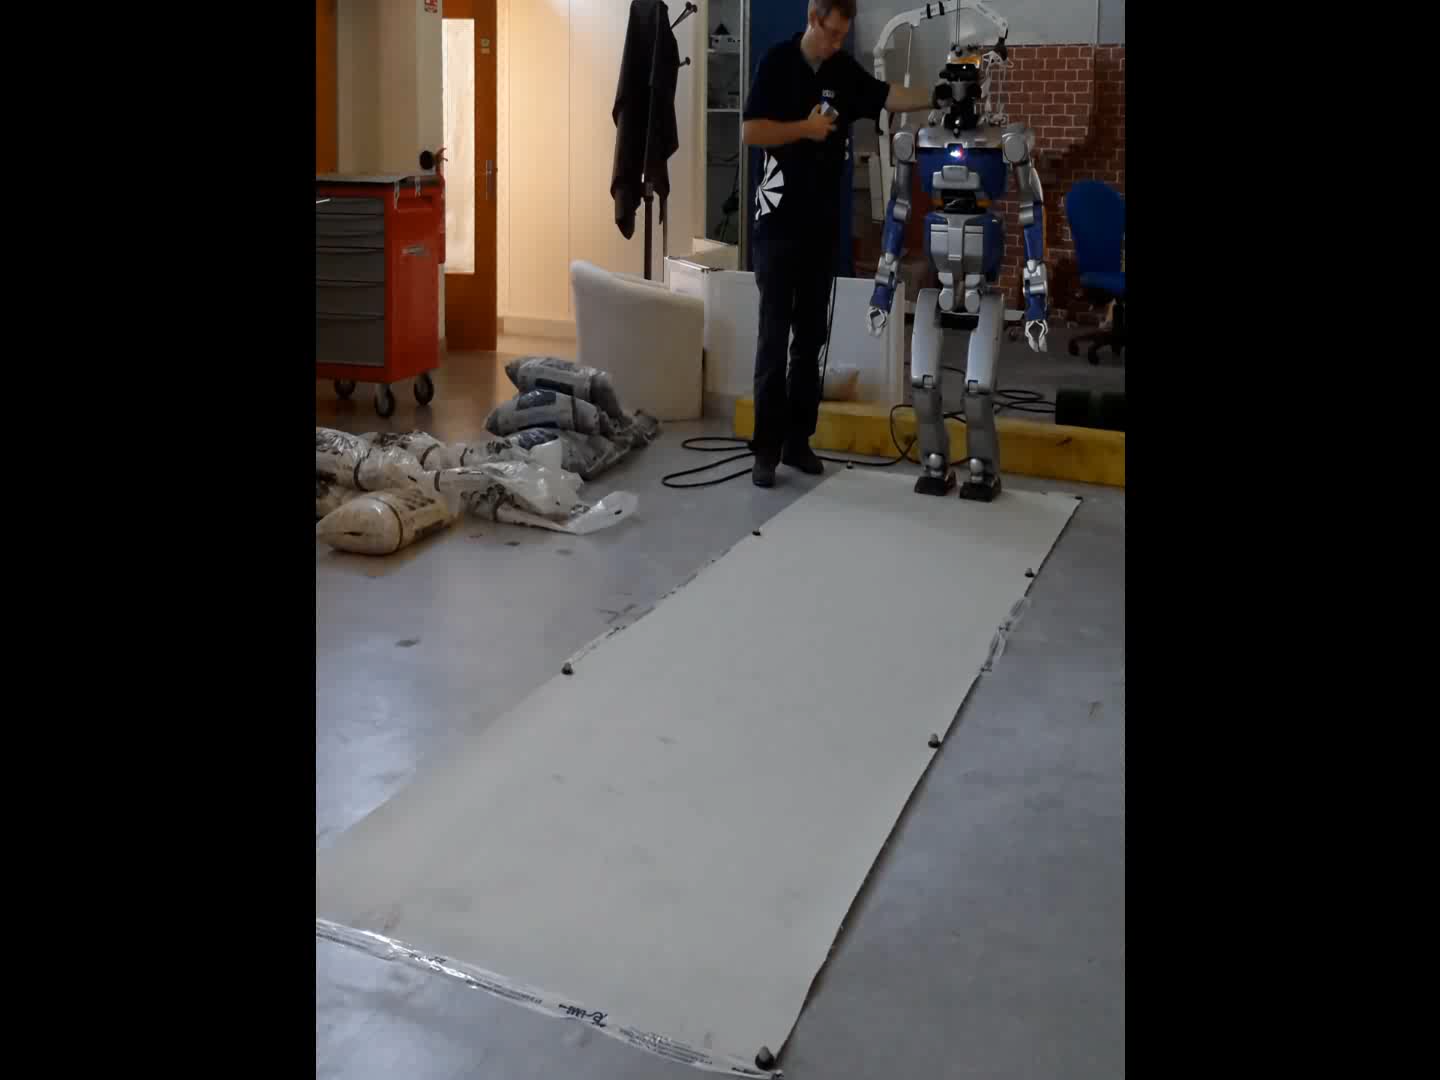
\includegraphics[width=0.3\linewidth, height=2.0cm]
      {koroibot/carpetkpi.png}    
    }  
    {./videos/Koroibot-carpet-rotate.mp4}
    
  \end{center}
\end{frame}
%%%%%%%%%%%%%%%%%%%%%%%%%%%%%%%%%%%%%%%%%%%%%%%%%%%%%%%%%%%%%%%%%%%%%%%%%%%%%%%%%%%%%%%%%%
\begin{frame}{Different Problematics}

\begin{itemize}
  \item flat ground walking [Herdt Advanced Robotics 2010]
  \begin{itemize}
    \item small step length ($5cm/step$)
    \item need planner for advanced application (like obstacle avoidance)
    \item important drift during rotation ($90deg$ in two laps of an ellipse)
  \end{itemize}
  
  \item stair walking
  \begin{itemize}
    \item important energy consumption ($5$ times more than flat ground walking)
  \end{itemize}
  
  \item beam walking
  \begin{itemize}
    \item no sensor feedback
  \end{itemize}
\end{itemize}
\only<2>{
\begin{tikzpicture}[remember picture, overlay]
  \draw [draw=red,sloped,line width=15pt,->] (0.5,0.5) -- node {\color{white}{\textbf{Reactivity \& Functionnality}}} (11.0,5.0);
\end{tikzpicture}
}
\end{frame}